\subsection{Results for Heading}
%\label{subsec:direction_results}
%\vspace{10pt}

Figure~\ref{fig:var_direction_RMSE} represents the $p$-values for the Wilcoxon signed-rank test on RMSE values across $k$-fold validation datasets for the heading in the $k$-fold testing datasets using different RNN models, and forecasting times. Darker colors in grayscale represent a higher $p$-value in a range from $0$ to $1$. The values on the secondary diagonal are all equal to $1$ and black because models equal themselves.

\begin{figure}[!ht]
	\centering
	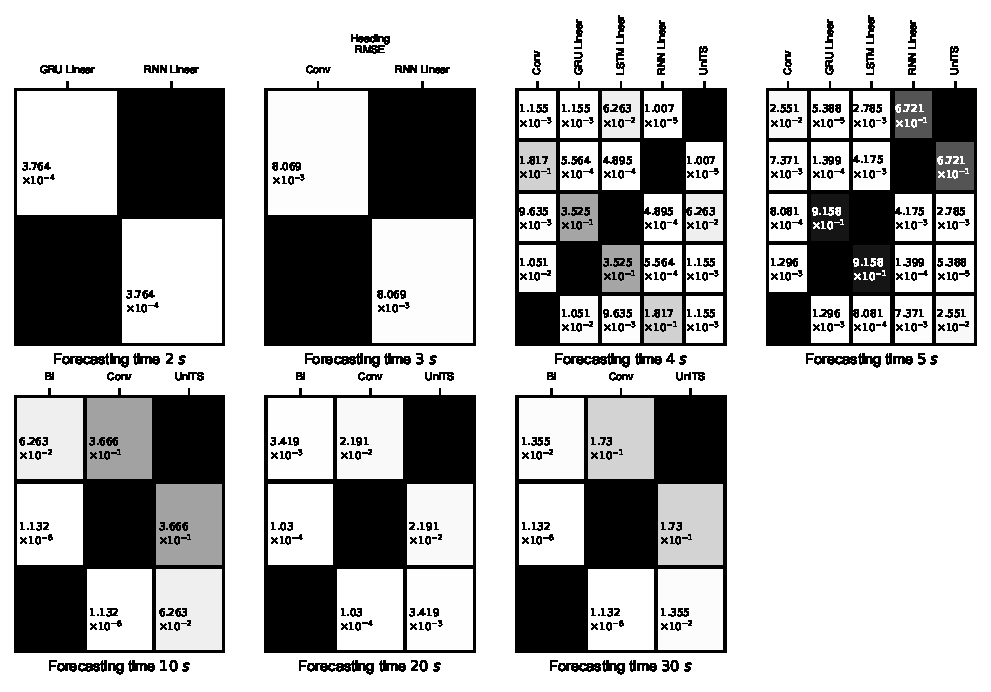
\includegraphics[width = 0.99 \linewidth]{var_direction_RMSE.pdf}
	\caption{The $p$-values for the Wilcoxon signed-rank test on RMSE values across $k$-fold validation datasets for the heading in the $k$-fold testing datasets using different RNN models, and forecasting times. Darker colors in grayscale represent a higher $p$-value in a range from $0$ to $1$. The values on the secondary diagonal are all equal to $1$ and black because models equal themselves.}
	\label{fig:var_direction_RMSE}
\end{figure}

Figure~\ref{fig:wilcoxon_RMSE_val_merged} contains the average RMSE across $k$-fold testing datasets using different validation datasets for all variables estimated in nested $k$-fold cross-validation by different RNN models, and forecasting times.

\begin{figure}[!ht]
	\centering
	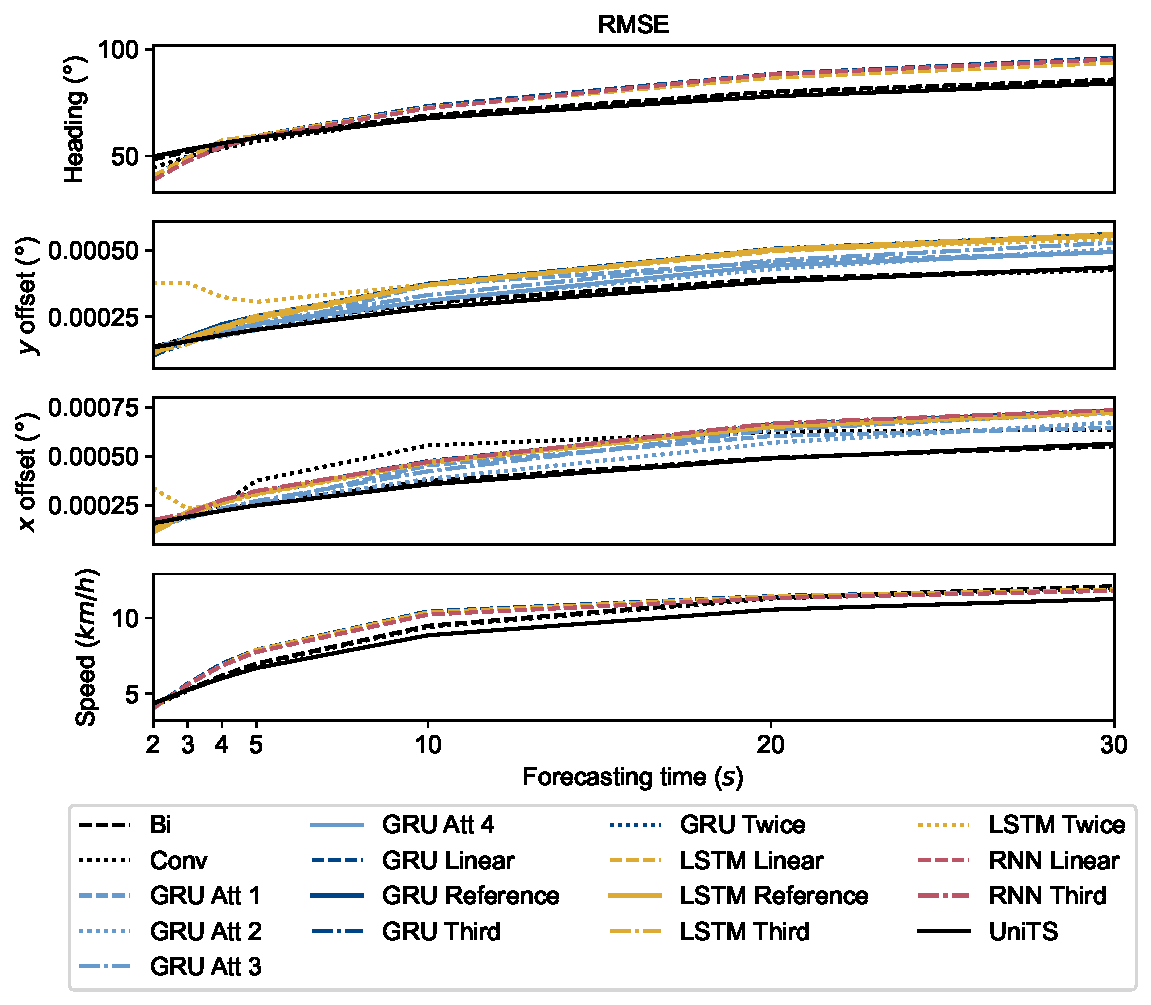
\includegraphics[width = 0.99 \linewidth]{wilcoxon_RMSE_val_merged.pdf}
	\caption{The average RMSE across $k$-fold testing datasets using different validation datasets for all variables estimated in nested $k$-fold cross-validation by different RNN models, and forecasting times.}
	\label{fig:wilcoxon_RMSE_val_merged}
\end{figure}

The average RMSE in $\degree$, with standard deviation in brackets, across $k$-fold validation datasets for the heading estimated on the $k$-fold testing datasets by different RNN models, and forecasting times is listed in Table~\ref{tab:wilcoxon_direction_RMSE}.

\begin{table}[!ht]
	\centering
	\resizebox{\linewidth}{!}{
		\begin{tabular}{|c|c|c|c|c|c|c|c|}
			\hline
			Model & $2$ $s$ & $3$ $s$ & $4$ $s$ & $5$ $s$ & $10$ $s$ & $20$ $s$ & $30$ $s$ \\ \hline
			\multirow{2}{*}{Bi} & $48.47$ & $52.16$ & $55.1$ & $59.02$ & $69.13$ & $80.22$ & $85.97$ \\
			 & ($2.35$) & ($2.31$) & ($2.21$) & ($2.58$) & ($2.11$) & ($2.4$) & ($2.49$) \\ \hline
			\multirow{2}{*}{Conv} & $44.62$ & $49.72$ & $\mathbf{53.58}$ & $\mathbf{56.94}$ & $68.41$ & $79.74$ & $84.99$ \\
			 & ($2.02$) & ($2.28$) & \textbf{(}$\mathbf{2.09}$\textbf{)} & \textbf{(}$\mathbf{2.26}$\textbf{)} & ($2.17$) & ($2.29$) & ($2.37$) \\ \hline
			\multirow{2}{*}{GRU Linear} & $40.55$ & $49.45$ & $55.29$ & $59.56$ & $73.51$ & $88.58$ & $96.2$ \\
			 & ($1.86$) & ($2.15$) & ($2.16$) & ($2.35$) & ($1.94$) & ($2.39$) & ($2.26$) \\ \hline
			\multirow{2}{*}{LSTM Linear} & $40.61$ & $49.2$ & $57.42$ & $59.47$ & $72.83$ & $86.76$ & $93.87$ \\
			 & ($2.43$) & ($2.05$) & ($9.67$) & ($2.34$) & ($2.21$) & ($1.87$) & ($2.2$) \\ \hline
			\multirow{2}{*}{RNN Linear} & $\mathbf{38.85}$ & $\mathbf{47.63}$ & $54.36$ & $58.71$ & $72.54$ & $88.35$ & $95.47$ \\
			 & \textbf{(}$\mathbf{1.85}$\textbf{)} & \textbf{(}$\mathbf{2.42}$\textbf{)} & ($2.22$) & ($2.05$) & ($2.33$) & ($1.93$) & ($2.48$) \\ \hline
			\multirow{2}{*}{UniTS} & $49.88$ & $53.14$ & $56.02$ & $58.6$ & $\mathbf{67.8}$ & $\mathbf{78.04}$ & $\mathbf{84.09}$ \\
			 & ($2.18$) & ($2.29$) & ($2.35$) & ($2.38$) & \textbf{(}$\mathbf{2.26}$\textbf{)} & \textbf{(}$\mathbf{2.29}$\textbf{)} & \textbf{(}$\mathbf{2.47}$\textbf{)} \\ \hline
		\end{tabular}
	}
	\caption{The average RMSE in $\degree$, with standard deviation in brackets, across $k$-fold validation datasets for the heading estimated on the $k$-fold testing datasets by different RNN models, and forecasting times.}
	\label{tab:wilcoxon_direction_RMSE}
\end{table}

The Conv model achieved the lowest RMSE for heading, and a forecasting time of $4$, and $5$ $s$ with average values and standard deviation (in brackets) that equal $53.58$ $\degree$ ($2.09$ $\degree$), and $56.94$ $\degree$ ($2.26$ $\degree$) respectively.

The Conv model does not have a statistically significantly different RMSE than the GRU Linear, LSTM Linear, RNN Linear, and UniTS models for heading using a forecasting time of $4$ $s$, with $p$-values equaling $1.051 \times 10^{-2}$, $9.635 \times 10^{-3}$, $1.817 \times 10^{-1}$, and $1.155 \times 10^{-3}$.

\markertable{tab:\label{tab:RMSE:direction:p:4}}

The Conv model does not have a statistically significantly different RMSE than the GRU Linear, LSTM Linear, RNN Linear, and UniTS models for heading using a forecasting time of $5$ $s$, with $p$-values equaling $1.296 \times 10^{-3}$, $8.081 \times 10^{-4}$, $7.371 \times 10^{-3}$, and $2.551 \times 10^{-2}$.

\markertable{tab:\label{tab:RMSE:direction:p:5}}

The RNN Linear model achieved the lowest RMSE for heading, and a forecasting time of $2$, and $3$ $s$ with average values and standard deviation (in brackets) that equal $38.85$ $\degree$ ($1.85$ $\degree$), and $47.63$ $\degree$ ($2.42$ $\degree$) respectively.

The RNN Linear model does not have a statistically significantly different RMSE than the GRU Linear model for heading using a forecasting time of $2$ $s$, with a $p$-value equaling $3.764 \times 10^{-4}$.

\markertable{tab:\label{tab:RMSE:direction:p:2}}

The RNN Linear model does not have a statistically significantly different RMSE than the Conv model for heading using a forecasting time of $3$ $s$, with a $p$-value equaling $8.069 \times 10^{-3}$.

\markertable{tab:\label{tab:RMSE:direction:p:3}}

The UniTS model achieved the lowest RMSE for heading, and a forecasting time of $10$, $20$, and $30$ $s$ with average values and standard deviation (in brackets) that equal $67.8$ $\degree$ ($2.26$ $\degree$), $78.04$ $\degree$ ($2.29$ $\degree$), and $84.09$ $\degree$ ($2.47$ $\degree$) respectively.

The UniTS model does not have a statistically significantly different RMSE than the Bi, and Conv models for heading using a forecasting time of $10$ $s$, with $p$-values equaling $6.263 \times 10^{-2}$, and $3.666 \times 10^{-1}$.

\markertable{tab:\label{tab:RMSE:direction:p:10}}

The UniTS model does not have a statistically significantly different RMSE than the Bi, and Conv models for heading using a forecasting time of $20$ $s$, with $p$-values equaling $3.419 \times 10^{-3}$, and $2.191 \times 10^{-2}$.

\markertable{tab:\label{tab:RMSE:direction:p:20}}

The UniTS model does not have a statistically significantly different RMSE than the Bi, and Conv models for heading using a forecasting time of $30$ $s$, with $p$-values equaling $1.355 \times 10^{-2}$, and $1.73 \times 10^{-1}$.

\markertable{tab:\label{tab:RMSE:direction:p:30}}

